% The document class supplies options to control rendering of some standard
% features in the result.  The goal is for uniform style, so some attention 
% to detail is *vital* with all fields.  Each field (i.e., text inside the
% curly braces below, so the MEng text inside {MEng} for instance) should 
% take into account the following:
%
% - author name       should be formatted as "FirstName LastName"
%   (not "Initial LastName" for example),
% - supervisor name   should be formatted as "Title FirstName LastName"
%   (where Title is "Dr." or "Prof." for example),
% - degree programme  should be "BSc", "MEng", "MSci", "MSc" or "PhD",
% - dissertation title should be correctly capitalised (plus you can have
%   an optional sub-title if appropriate, or leave this field blank),
% - dissertation type should be formatted as one of the following:
%   * for the MEng degree programme either "enterprise" or "research" to
%     reflect the stream,
%   * for the MSc  degree programme "$X/Y/Z$" for a project deemed to be
%     X%, Y% and Z% of type I, II and III.
% - year              should be formatted as a 4-digit year of submission
%   (so 2014 rather than the academic year, say 2013/14 say).

\documentclass[ % the name of the author
                    author={James Stephenson},
                % the name of the supervisor
                supervisor={Dr. Edwin Simpson},
                % the degree programme
                    degree={MSc},
                % the dissertation    title (which cannot be blank)
                     title={Project Plan: Bayesian Deep Learning For Extractive Test Summarisation},
                % the dissertation subtitle (which can    be blank)
                  subtitle={},
                % the dissertation     type
                      type={},
                % the year of submission
                      year={2022}]{../additions/dissertation}

\begin{document}

	% =============================================================================
	
	
	% =============================================================================
	
	% This macro creates the standard UoB title page by using information drawn
	% from the document class (meaning it is vital you select the correct degree 
	% title and so on).
	
	
	\maketitle
	
	% After the title page (which is a special case in that it is not numbered)
	% comes the front matter or preliminaries; this macro signals the start of
	% such content, meaning the pages are numbered with Roman numerals.
	
	\frontmatter
	
	% LaTeX automatically generates a table of contents, plus associated lists 
	% of figures, tables and algorithms.  The former is a compulsory part of the
	% dissertation, but if you do not require the latter they can be suppressed
	% by simply commenting out the associated macro.
	
	\tableofcontents
	
	% The following sections are part of the front matter, but are not generated
	% automatically by LaTeX; the use of \chapter* means they are not numbered.
	
	% -----------------------------------------------------------------------------
	
	\chapter*{Abstract}		

		Text summarisation is a valuable technique that allows for the computational processing of documents, saving readers hours in manual processing. Users have different summary requirements; however, current extractive summarisation systems construct generic summaries that are not tailored to the user's needs. Asking users for feedback is one solution to combat this problem, yet this introduces an additional step of manual processing. Thus, we look to minimise the amount of required user feedback.

		\medbreak	
		This project will investigate the feasibility of applying newly-developed techniques from Bayesian deep learning \cite{Wilson20} to get significant estimates of the model's confidence, so we can ask the user for more explanatory feedback. Legacy approaches use Bayesian optimisation \cite{Simpson19} strategies the achieve minimal user feedback; however, this strategy is blocked since modern summarisation techniques involve deep neural networks which cannot effectively express uncertainty and are typically overconfident when encountered by new topics \cite{Xu19}. This poses an issue in utilising the feedback strength of Bayesian optimisation.

		\medbreak		
		Specifically, we look to utilise pre-trained deep learning models such as BERT to ascertain instances in a vector format to be used in an active learning component. Monte-Carlo Dropout \cite{Gal15} techniques appear to be proficient approximations for parameter posterior distributions. Thus, we will look to utilise this approach to calibrate our model.

		\medbreak
		It is common in passage ranking active learning solutions to use a pool-based strategy to query unlabelled instances \cite{EinDor20}. However, this requires excess computational processing. Thus, we look to use a stream-based approach to identify instances to query since it provides a lighter framework for an interactive setting. Query-by-committee acquisition functions are popular for stream-based active learning; however, since Simpson et al. \cite{Simpson19} found Bayesian optimisation strategies effectively minimised user feedback, we will look to utilise strategies such as expected improvement since Bayesian deep learning will provide a higher level of model confidence. 

		
		
	
	\mainmatter
	
	% -----------------------------------------------------------------------------
	 
	\chapter{Two Pages of Coherent Text: An Introduction}
	\label{chap:introduction}
		
		It should include at least two pages of coherent text (i.e., of the form you intend to write for your thesis, not rough-notes) that could be used as the opening pages of your Introduction/Overview chapter (Chapter 1 of your thesis). 
		
	% -----------------------------------------------------------------------------
	
	\chapter{Subject Background}
	\label{chap:literaturereview}
		
	Since the crux of this project is to assess the suitability of applying Bayesian deep learning (BDL) techniques to passage ranking (PR) problems, this chapter explores the relevant literature that discusses previous approaches to passage ranking solutions. Once this assessment has been done, we will then also examine literature that assesses BDL as opposed to classical deep learning techniques.
		
		\section{Interactive Learning}
		\label{chap:literaturereview:interactive}
		
		Interactive learning is a machine learning workflow involving directed experimentation with inputs and output \cite{Amershi14}. A rapid change in response to user input facilitates interactive inspection of the impact of the user’s input.  This workflow format is commonly used to solve NLP problems; related works include literature in passage ranking (PR) of generated text in the context of translations, question answering and text summarisation \cite{Peris18, Lin17, PVS17}. These works had a focus on interactionally-expensive uncertainty sampling to learn the rankings of \emph{all} candidate passages \cite{Simpson19}. Gao et al. \cite{Gao18} researched how to reduce the number of user interactions for uncertainty sampling techniques with some success using an active learner. A positive step towards reasonable interactive learning.

\medbreak
Simpson et al \cite{Simpson19} take an alternative approach to uncertainty sampling by proposing a Bayesian optimisation (BO) strategy instead \cite{Simpson19}. With Gaussian process (GPs) displaying some success in error reduction for NLP tasks with noisy labels \cite{Cohn13, Beck14}, Simpson and Gurevych \cite{Simpson18} proposed using Gaussian process preference learning (GPPL) with uncertainty sampling. This approach has been further built upon by Simpson et al. \cite{Simpson19} to a BO framework. This approach showed a markable improvement in the accuracy of chosen answers in a community question answering (cQA) task with a small number of interactions required \cite{Simpson19}. The methodology used Expected Improvement (IMP) as the acquisition function for AL which twisted the focus of optimisation to find the best candidate, as opposed to the ranks of all candidates \cite{Simpson19}. The switch to the exploitation of promising candidates showed to be massively influential on performance \cite{Simpson19}. Simpson et al. \cite{Simpson19} furthered the performance enhancement gained from using the BO framework by using prior predictions from a deep learner as an informative prior for GPPL \cite{Simpson19} to address the cold-start problem for recommender systems \cite{Bobadilla12}.

		
		\section{Active Learning}
		\label{chap:literaturereview:active}
		
		Alongside unsupervised and supervised learning, active learning (AL) is a machine learning framework whereby queries are asked of an oracle – such as a human annotator – in the form of labelling unlabelled observations \cite{Settles09}. The active interactions with oracles allow better performance with few labelled data points. AL is beneficial in the cases where labelled data is scarce due to high costs; for speech recognition problems \cite{Zhu05} details a scale factor of ten times between the length of a speech extract and the time taken to annotate such as extract.
		
			\subsection{Active Learning Strategies}
			\label{chap:literaturereview:active:strategies}
			
			Settles \cite{Settles09} describes three scenarios that are considered in the literature to categorise AL problems: Membership query synthesis, Stream-based selective sampling and pool-based active learning.

			\paragraph{Membership query synthesis.}  Labels are requested by the learner for any unlabelled instance in the input space. This includes queries that are generated as if for the first time rather than from some causal distribution \cite{Angluin88}. A considerable limitation of this scenario occurs when the oracle is a human annotator. Baum and Lang \cite{Baum92} employed membership query learning to classify handwritten characters using a human oracle. They found that many query images that were generated were unrecognisable symbols. This limitation could feasibly produce nonsense summaries when tasked with a PR situation; something we should be cautious of.

			\paragraph{Stream-based selective sampling.} In this setting, unlabelled observations are selected sequentially and the learner determines whether to query or discard each instance; this is done to reduce annotation effort \cite{Cohn94}. This is under the major assumption that acquiring unlabelled instances is low-cost since the learner needs to be able to decide it can discard the unlabelled observation with minimal opportunity cost. The most common way of defining if a sample should be queried or discarded is by creating a \emph{version space} \cite{Mitchell82} using two models with different parameter choices; for those instances that the models agree on, we can discard as there is little uncertainty. However, with regards to the cases of disagreement, these unlabelled instances fall in the region of uncertainty \cite{Settles09}. This region of uncertainty is computationally expensive to calculate; thus, it is common to use approximations in practice \cite{Seung92, Cohn94, Dasgupta07}.

			\paragraph{Pool-based active learning.} A common approach for many real-world examples such as text classification \cite{Lewis94}, information extraction \cite{Thompson99} and speech recognition \cite{Tur05} since it is common to find large groups of unlabelled data collected at once. The \emph{pool-based active learning} workflow starts with a learner trained on a small set of labelled data, $ \mathcal{D}_{lab} $, which is then used to \emph{greedily} rank instances in a large collection of unlabelled instances, $\mathcal{D}_{unlab} $ \cite{Lewis94}. The highest-ranked instance is then labelled by an oracle and then used within the learner retrain. In comparison to a stream-based active learner, a greater computational cost is associated with a pool-based learner since it ranks the entire set $\mathcal{D}_{unlab}$ before making a query as opposed to making sequential decisions.
	
		\subsection{Acquisition Functions}
		\label{chap:literaturereview:active:acquisition}
		
			Whilst introducing \emph{active learning}, a lot is spoken about measuring the usefulness of each instance and whether to query it or not. We measure how informative an instance is using \emph{acquisition functions}. Naturally, there is a trade-off between two types of approaches: exploration and exploitation. Exploitative strategies search the area of the current best instances; whereas exploration strategies look at instances that have greater levels of uncertainty. As expected, there are many acquisition functions currently researched; we will cover a few important ones from the areas of uncertainty sampling and Bayesian optimisation.

			\paragraph{Uncertainty Sampling.} Posed by Lewis and Gale \cite{Lewis94}, it is an explorative query framework which focuses on querying instances that have the most uncertainty. A common strategy used to calculate uncertainty for binary, probabilistic learning models is by using Shannon’s entropy \cite{Shannon48} given by the formula below.

	$$
		x^{\ast}_{ENT} = argmax_{x} - \sum_i \mathbb{P}(y_i \mid x; \omega) log \left[ \mathbb{P}(y_i \mid x; \omega) \right]
	$$
	
		\noindent
		for $y_i$ across the range of possible labels; in the context of whether to query or not, $y_i \in {0,1}$ since we have a binary decision to make. Entropy-based acquisition functions have been generalised for more complex models so they are suitable for tree-based or multi-label classification models \cite{Craven08, Hwa04}. However, uncertainty sampling suffers from a lack of sensitivity to noise and outliers as it can get very easily distracted. Uncertainty sampling also does not consider why the model holds uncertainty for a particular instance \cite{Sharma17}.

		\paragraph{Expected Improvement (EI).} This is an alternative, Bayesian optimisation approach that has a deeper focus on the exploitation of good instances \cite{Mockus75}. The basic idea is that it provides an estimation of the \emph{expected improvement} of a proposed candidate over our current best candidate. Simpson et all \cite{Simpson19} find this an effective acquisition function for their interactive passage ranking model with a minimal number of user interactions. To outline how we calculate EI, we must first define \emph{improvement} as $max\{0, f_a - f_b\}$ with $a$ our candidate instance, $b$ our current best instance, and $f$ the utility of a given instance \cite{Simpson19}. The first assumption we make is that $\mathcal{N}(\hat{f}, \mathcal{C})$ is a good estimate for the posterior distribution of candidate utilities; second that the difference in utilities $f_a - f_b$ is Gaussian-distributed. With these assumptions, can derive the following equation for expected improvement with $z = \frac{\hat{f}_a - \hat{f}_b}{\sqrt{v}}$ and posterior standard deviation $\sqrt{v}$:

		$$
			Imp(a; \mathcal{D}) = \sqrt{v}\left[z \Phi(z) + \mathcal{N}(z; 0, 1)\right]
		$$	

\noindent
Some limitations of EI is that it has been found to over-exploit in some cases \cite{Qin17}; since it takes a very exploitative sample, if there are inaccuracies in the estimation of the mean or variance, it does not have the explorative capabilities to find the optimal instance area.

\paragraph{Query-By-Committee (QBC).} This acquisition function utilises a committee of models with different parameters, ${\omega^1, \ldots, \omega^{c}}$, that are all trained on the same labelled dataset \cite{Seung92}. Optimal research size has been researched; however, even a committee size of two or three models has shown positive results in practice \cite{Seung92, Craven08, Nigam98} providing no agreement on an appropriate committee size. QBC looks for instances that the models disagree on, making this acquisition function have a strong emphasis on exploration. It is a common acquisition function for stream-based learning \cite{Settles09} as it does not require a batch of unlabelled instances to make a decision. QBC does require a measure of disagreement among committee models. The two main approaches are \emph{vote entropy} and \emph{average Kullback-Leibler (KL) divergence}. 

		\paragraph{Vote Entropy (VE).} is a QBC generalisation of entropy-based uncertainty sampling, defined by the following structure \cite{Dagan95}:

		$$
			x^\ast_{VE} = argmax_x - \sum_i \frac{V(y_i)}{\mathcal{C}} log \left[\frac{V(y_i)}{\mathcal{C}}\right]
		$$
		
		\noindent
		where $y_i$ ranges across all possible labels and $V(y_i)$ is the number of votes that the instance receives to be assigned label $i$.

		\paragraph{Average KL divergence} is built on KL divergence \cite{Kullback51} to measure the average difference between two probability distributions as detailed below \cite{Nigam98}:

		$$
			x^\ast_KL = argmax_x \frac{1}{\mathcal{C}} \sum_{c=1}^{\mathcal{C}} \sum_i \mathbb{P}(y_i \mid x; \omega^{c}) log \left[\frac{\mathbb{P}(y_i \mid x; \omega^{c})}{\mathbb{P}(y_i \mid x; \mathcal{C}}\right]
		$$

\noindent
where $\omega^{(c)}$ represents the parameters of a particular model in the committee, $\mathcal{C}$ represents the committee as a whole.

\medbreak
Average KL divergence is known to miss some instances when committee members disagree where VE does not whereas, a limitation of VE is that it can miss informative instances \cite{Li06}. A shared weakness is that both metrics often fail to select enough valuable instances to achieve the same classification accuracy as passive learning.

		
		
		\section{Deep Learning}
		\label{chap:literaturereview:deep}
		
		Deep learning methods form a subset of machine learning, based on neural networks with at least three hidden layers. These techniques have dramatically increased the capabilities of model recognition in many domains including visual object recognition, question answering and text summarisation \cite{Lecun15, Sharma18, Azar17}. In classical training, one typically uses maximum a-posteriori (MAP) optimisation to choose the set of parameters, $\hat{w}$, for our model that maximises the posterior probability from our parameter distribution \cite{Wilson20}. MAP does not require computationally-costly calculations of the marginal distribution \cite{Hero15}; however, since MAP is a point estimate, it cannot be fully considered a Bayesian approach \cite{Hero15}.

		\begin{figure}
			\centering
			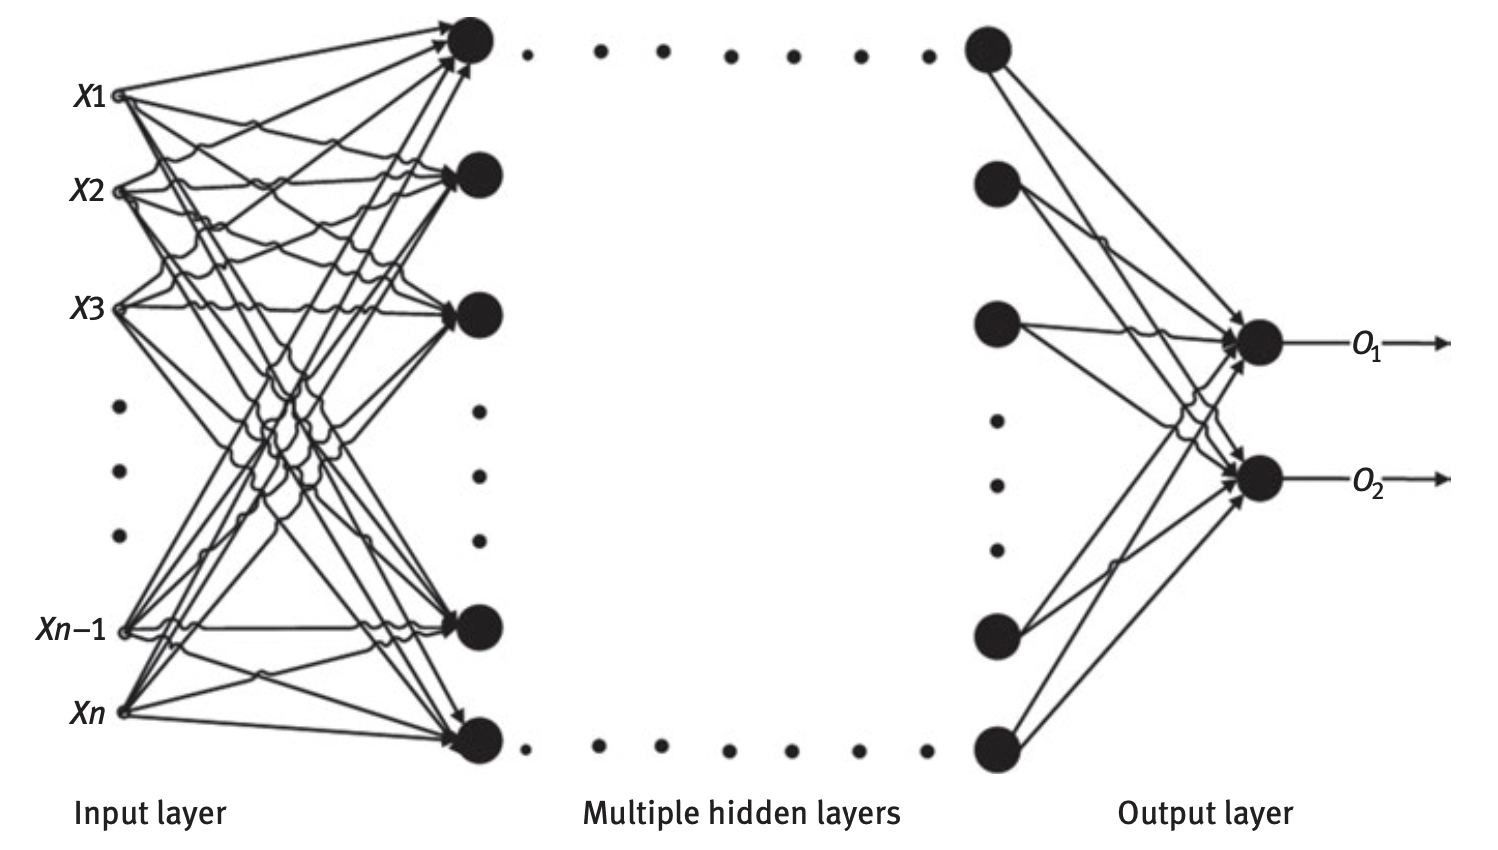
\includegraphics[width=0.5\linewidth]{../additions/figures/Bhattacharyya20_plot_Deep}
			\caption{Typical deep learning architecture \cite{Bhattacharyya20}}
			\label{fig:deep_architecture}
		\end{figure}
		
			\subsection{Pre-trained Models}
			\label{chap:literaturereview:deep:pretrained}
			
			Pre-trained, deep learning, language models are useful in unsupervised learning problems due to the lack of major architectural modifications required and the high-performance levels that are delivered \cite{Mridha21}. One popular pre-trained language model is the Bidirectional Encoder Representations from Transformers (BERT) which takes an entire sequence of words, bidirectionally, to produce significantly improved results. The input is augmented by three embeddings – position, segment and token embeddings – and padded by a [CLS] token at the beginning of the first sentence to ensure BERT has lots of useful information \cite{Navin21}.
			
			\medbreak
			BERT is trained on two tasks in parallel: Masked Language Modelling, prediction of hidden words in sentences, and Next Sentence Prediction \cite{Navin21}. However, BERT can be applied to many NLP tasks \cite{Mridha21} such as question answering and text classification tasks with some minor fine-tuning; we add a small layer on the top of the transformer output for the [CLS] token \cite{Navin21} to adapt the core model to different tasks. Recent publications have found BERT-based models \cite{Devlin18} to be extremely effective when tasked with passage ranking situations across the question answering and text summarisation disciplines \cite{Xu19, Qiao19}. Xu et al. \cite{Xu19} explored a query-passage set-up when applying BERT to cQA such that the BERT final hidden state fed into an MLP module to produce relevance scores in a supervised way. Since this technique outperformed the baseline, it may be a useful structure to consider adapting to the text summarisation domain.
			
			\medbreak
			The limitation of utilising an interactive learning framework such as one outlined by Simpson et al. \cite{Simpson19} is that it does not utilise the vast performance capabilities of newer, pre-trained techniques such as BERT. Although the framework presented does limit the number of interactions required from a user – allowing the user to tailor the summary – Ein-Dor et al. \cite{EinDor20} look to take this idea further with the incorporation of a BERT component in an AL framework. 		
		
		\section{Bayesian Deep Learning}
		\label{chap:literaturereview:deepbayes}
		
			Bayesian Deep Learning is a deep learning approach which uses a probabilistic framework – whether that be in the model acquisition function or model parameters – to improve model performance. Bayesian acquisition functions are something we have mentioned previously; however, concerning a probabilistic approach to the selection of model parameters, $\omega$, marginalisation is used to replace optimisation. This is so we can utilise the effect of several models using different $\omega$ with probability distribution $p(\omega)$. To allow us to marginalise over $\omega$, we require Bayes Theorem to link the \emph{prior distribution}, $p(\omega)$, for parameters $\omega$; the likelihood, $p(\mathcal{D} \mid \omega)$ of such parameters being suitable for data, $\mathcal{D}$; and the \emph{posterior distribution}, $p(\omega \mid \mathcal{D})$, of the parameters.
		
		$$
			p(\omega \mid \mathcal{D}) = \frac{p(\mathcal{D}_y \mid  \mathcal{D}_x, \omega)p(\omega)}{\int_{\omega'} p( \mathcal{D}_y \mid  \mathcal{D}_x, \omega')p(\omega')d\omega'}
		$$
	
		\noindent
		The marginalisation stage forms the integral over all possible $\omega$ on the numerator. The posterior distribution is incredibly useful to calculate the predictive distribution (or marginal probability distribution) of the output. The \emph{predictive distribution}, $p(y \mid \mathcal{D}, x)$, defines the probability of label $y$ given additional input $x$ and dataset  $\mathcal{D}$ \cite{Izmailov20}.
		
		$$
			p(y \mid x,  \mathcal{D}) = \int_\omega p(y \mid x, \omega)p(\omega \mid  \mathcal{D}) d\omega
		$$
		
		\noindent
		This integral is called \emph{Bayesian Model Averaging (BMA)} and can be thought of as the weighted average (using probability distributions) of all parameters and defines the probability for label $y$ given input $x$ and data $\mathcal{D}$ \cite{Izmailov20}. Wilson and Izmailov \cite{Izmailov20} argue that using a BMA increases accuracy as well as obtaining a realistic expression of uncertainty with classical neural networks exhibiting overconfident predictions \cite{Xu19}. Unfortunately, calculating the posterior distribution is a computationally expensive task, due to the marginalisation step in the denominator, so approximate posterior distributions are used.
		
			\subsection{Bayesian Deep Learning Strategies}
			\label{chap:literaturereview:deepbayes:strategies}
			
			Firstly, Wilson and Izamailov \cite{Izmailov20} comment that taking a selection of possible $\omega$ and combining the resulting models to approximate BMA – named Monte Carlo approximation – evocative of frequentist deep ensembles. However, there are modern approaches one can take.
			
			\medbreak
			A common practical method is using Monte Carlo Markov Chains (MCMC) to approximate the posterior \cite{Izmailov20}. MCMCs are used to approximate variable distributions for an idealised system \cite{Brooks11} and two common algorithms have been tailored to approximate posterior distributions: Gibbs Sampling and the Metropolis-Hastings Algorithm. However, Gibbs Sampling is not appropriate for neural networks with conditional posterior distributions due to the interdependency of parameters \cite{Neal95}. Simple forms of the Metropolis-Hasting algorithm (MH) can be more appropriate; however, again due to the high interdependence of states, MH can be costly and prone to random walks. Duane et al. \cite{Duane87} propose an alternative \emph{hybrid Monte Carlo} which is a combination of MH with sampling techniques from dynamical simulation.
			
			\medbreak
			Second, Graves \cite{Graves11} proposed fitting a Gaussian variational posterior approximation over the parameters of neural networks and optimising over the parameters to ensure the variational distribution is as good an estimate of the posterior distribution as possible. This method works well for networks of moderate size, but supplies training difficulties when working with larger architectures \cite{He15}.
Thirdly, Gal and Ghahramani \cite{Gal15} present Monte Carlo Dropout (MC Dropout); a dropout framework which integrates stochasticity into a neural network, by randomly removing parameters \emph{during training}. We can interpret dropout as approximate Bayesian inference, leading to a range of difference parameters. It is intuitive to see the link between this and sampling parameters from a posterior to approximate a predictive distribution.
		
			\begin{figure}
				\centering
				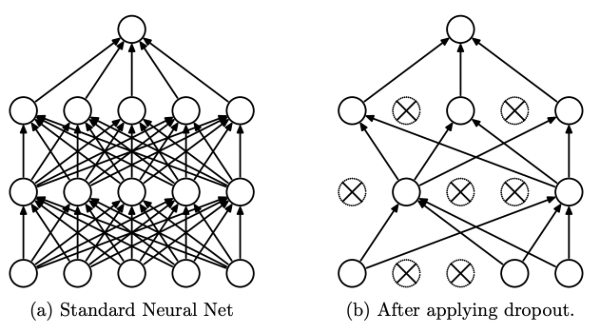
\includegraphics[width=0.5\linewidth]{../additions/figures/Srivastava14_MCDropout}
				\caption{Neural Network undergoing Monte Carlo Dropout \cite{Srivastava14}}
				\label{fig:MC_dropout}
			\end{figure}
			
			\medbreak
			Denoting the neural network parameter matrices for layer $i$ as $W_i$ alongside input and output sets $\mathcal{D}_{in}, \mathcal{D}_{out}$, we again suffer from an intractable posterior distribution $p(y \mid x, \mathcal{D}_{out}, \mathcal{D}_{in})$. Thus $q(\omega)$ is an approximation defined below
			
			\begin{align*}
				z_{i, j} &\sim Bernoulli(p_i) \\
				W_i &= M_i \cdot diag(z_{i,j})
			\end{align*}
			
			\noindent
			A simple Bernoulli distribution is used to determine which states are set to zero given some probability $p_i$ and variational parameters $M_i$. Note here that $z_{i,j}$ denotes unit $j$ in layer $i-1$.
			
			\medbreak
			To obtain the model uncertainty obtained through dropout in neural networks, we take our approximate predictive distribution. Through $T$ sample sets of realisations from our posterior distribution $z_{i,j}$, we get $T$ parameter matrices $\{W^{t}_{1}, W^{t}_{2}, \ldots W^{t}_{L}\}^{T}_{t=1}$, we get the following estimate by which we call our Monte Carlo Dropout.
			
			$$
				\mathbb{E}_{q(y^\ast \mid x^\ast)}(y^\ast) \approx \frac{1}{T} \sum_{t=1}^{T} \hat{y}^\ast(x^\ast, W_{1}^{t}, \ldots, W_{L}^{t})
			$$
			
			Another popular technique is \emph{Stochastic Weight Averaging – Gaussian (SWAG)} \cite{Maddox19}. This builds on the idea of \emph{Stochastic Weight Averaging (SWA)} which combines parameters of the same neural network at different stages in training \cite{Dmitrii18}. SWAG uses Stochastic Gradient Descent (SGD) information to estimate the shape of the posterior distribution by fitting a Gaussian distribution to the first two moments of the SGD iterate \cite{Maddox19}. We use these fitted Gaussian distributions for BMA. The benefits of SWAG are grounded in its practicality, stability and accuracy which are essential attributes when working with large neural networks \cite{Maddox19}.

			
		\section{Deep Active Learning}
		\label{chap:literaturereview:deepactive}
		
		Ideally, our solution would retain the AL component that exists in the PR framework proposed by Simpson et al \cite{Simpson19} since it allows us to tailor generated summaries to the user preferences; an essential aspect of summary ranking.
		
		\medbreak
		Zhang and Zhang also explored an ensemble of AL strategies to build a deep active learning framework \cite{Zhang19}. This was a composition of a BERT-based classifier and an ensemble sampling method to choose valuable data for training. They found that this alternative approach only required half the training data to attain state-of-the-art performance. However, the framework proposed by Ein-Dor et al. \cite{EinDor20} may be of more use since experimentation was constructed on data with high class imbalance, scarce labelling and a small annotation budget: attributes of an interactive PR context.  
		
		\medbreak
		Ein-Dor et al. \cite{EinDor20} developed a framework that used an AL approach with BERT-based classification. This structure consisted of pool-based AL in batch mode in conjunction with BERT as the classification scheme. Different AL strategies were examined – Monte-Carlo Dropout (MC DROPOUT) \cite{Gal15}, a Bayesian approach and Discriminative Active Learning (DAL) \cite{Gissin19} – with Al proving an excellent boost to helping BERT emerge from its poor initial model \cite{EinDor20}. Although DAL would not be appropriate for the PR context due to its focus on querying batches, using MC Dropout as a strategy seems to be effective for PR.
		
		\medbreak
		Gal and Ghahramani \cite{Gal17} also present an AL framework which incorporates recent Bayesian deep learning techniques. AL is limited by its ability to scale to high-dimensional datasets \cite{Tong01}, key for deep learning scenarios. Thus, Gal and Ghahramani proposed an approach that used specialised Bayesian convolutional neural networks (BCNNs) whereby Gaussian, prior probability distributions are used to describe a set of parameters as a basepoint to start inference. Like Ein-Dor et al., they also introduce MC Dropout to sample the approximate posteriors; however, Gal and Ghahramani do take a different approach by using the BALD acquisition function \cite{Houlsby11}. BALD chooses pool sizes with the greatest expectation of the information gained from the model parameters \cite{Gal17}; chosen since it demonstrates a small test error in experimentation.

		\section{Text Summarisation Models}
		\label{chap:literaturereview:summodels}
		
		We will start by discussing some of the text summarisation methods that we intend to use for this project; since this is not the central focus of our research, it suffices to use an off-the-shelf solution. Simpson et al \cite{Simpson19} simply take random sentences from the base text to create summaries which they found to be a sufficient approach to test their proposed PR framework since it is lightweight and can produce test summaries quickly. However, a modern, abstractive model that is likely to produce more realistic summaries for popular use such as Google’s Pegasus model \cite{Zhao19} would be a positive alternative. There are downsides to using such a model; namely, the model size will increase the computational cost of attaining instances and, since it is a pre-trained deep learning model, there could be a limitation on the number of parameter adjustments one can make for approaches such as Query-By-Committee.
		
		% ----------------------------------------------------------------------------	
	
	% =============================================================================
	
	% Finally, after the main matter, the back matter is specified.  This is
	% typically populated with just the bibliography.  LaTeX deals with these
	% in one of two ways, namely
	%
	% - inline, which roughly means the author specifies entries using the 
	%   \bibitem macro and typesets them manually, or
	% - using BiBTeX, which means entries are contained in a separate file
	%   (which is essentially a database) then imported; this is the 
	%   approach used below, with the databased being dissertation.bib.
	%
	% Either way, the each entry has a key (or identifier) which can be used
	% in the main matter to cite it, e.g., \cite{X}, \cite[Chapter 2}{Y}.
	
	\backmatter
	
	\bibliography{bibtex}
	
	% -----------------------------------------------------------------------------
	
	% The dissertation concludes with a set of (optional) appendices; these are 
	% the same as chapters in a sense, but once signalled as being appendices via
	% the associated macro, LaTeX manages them appropriately.
	
	\appendix
	
	\chapter{Time-plan}
		\label{appx:timeplan}
		
		\begin{center}
			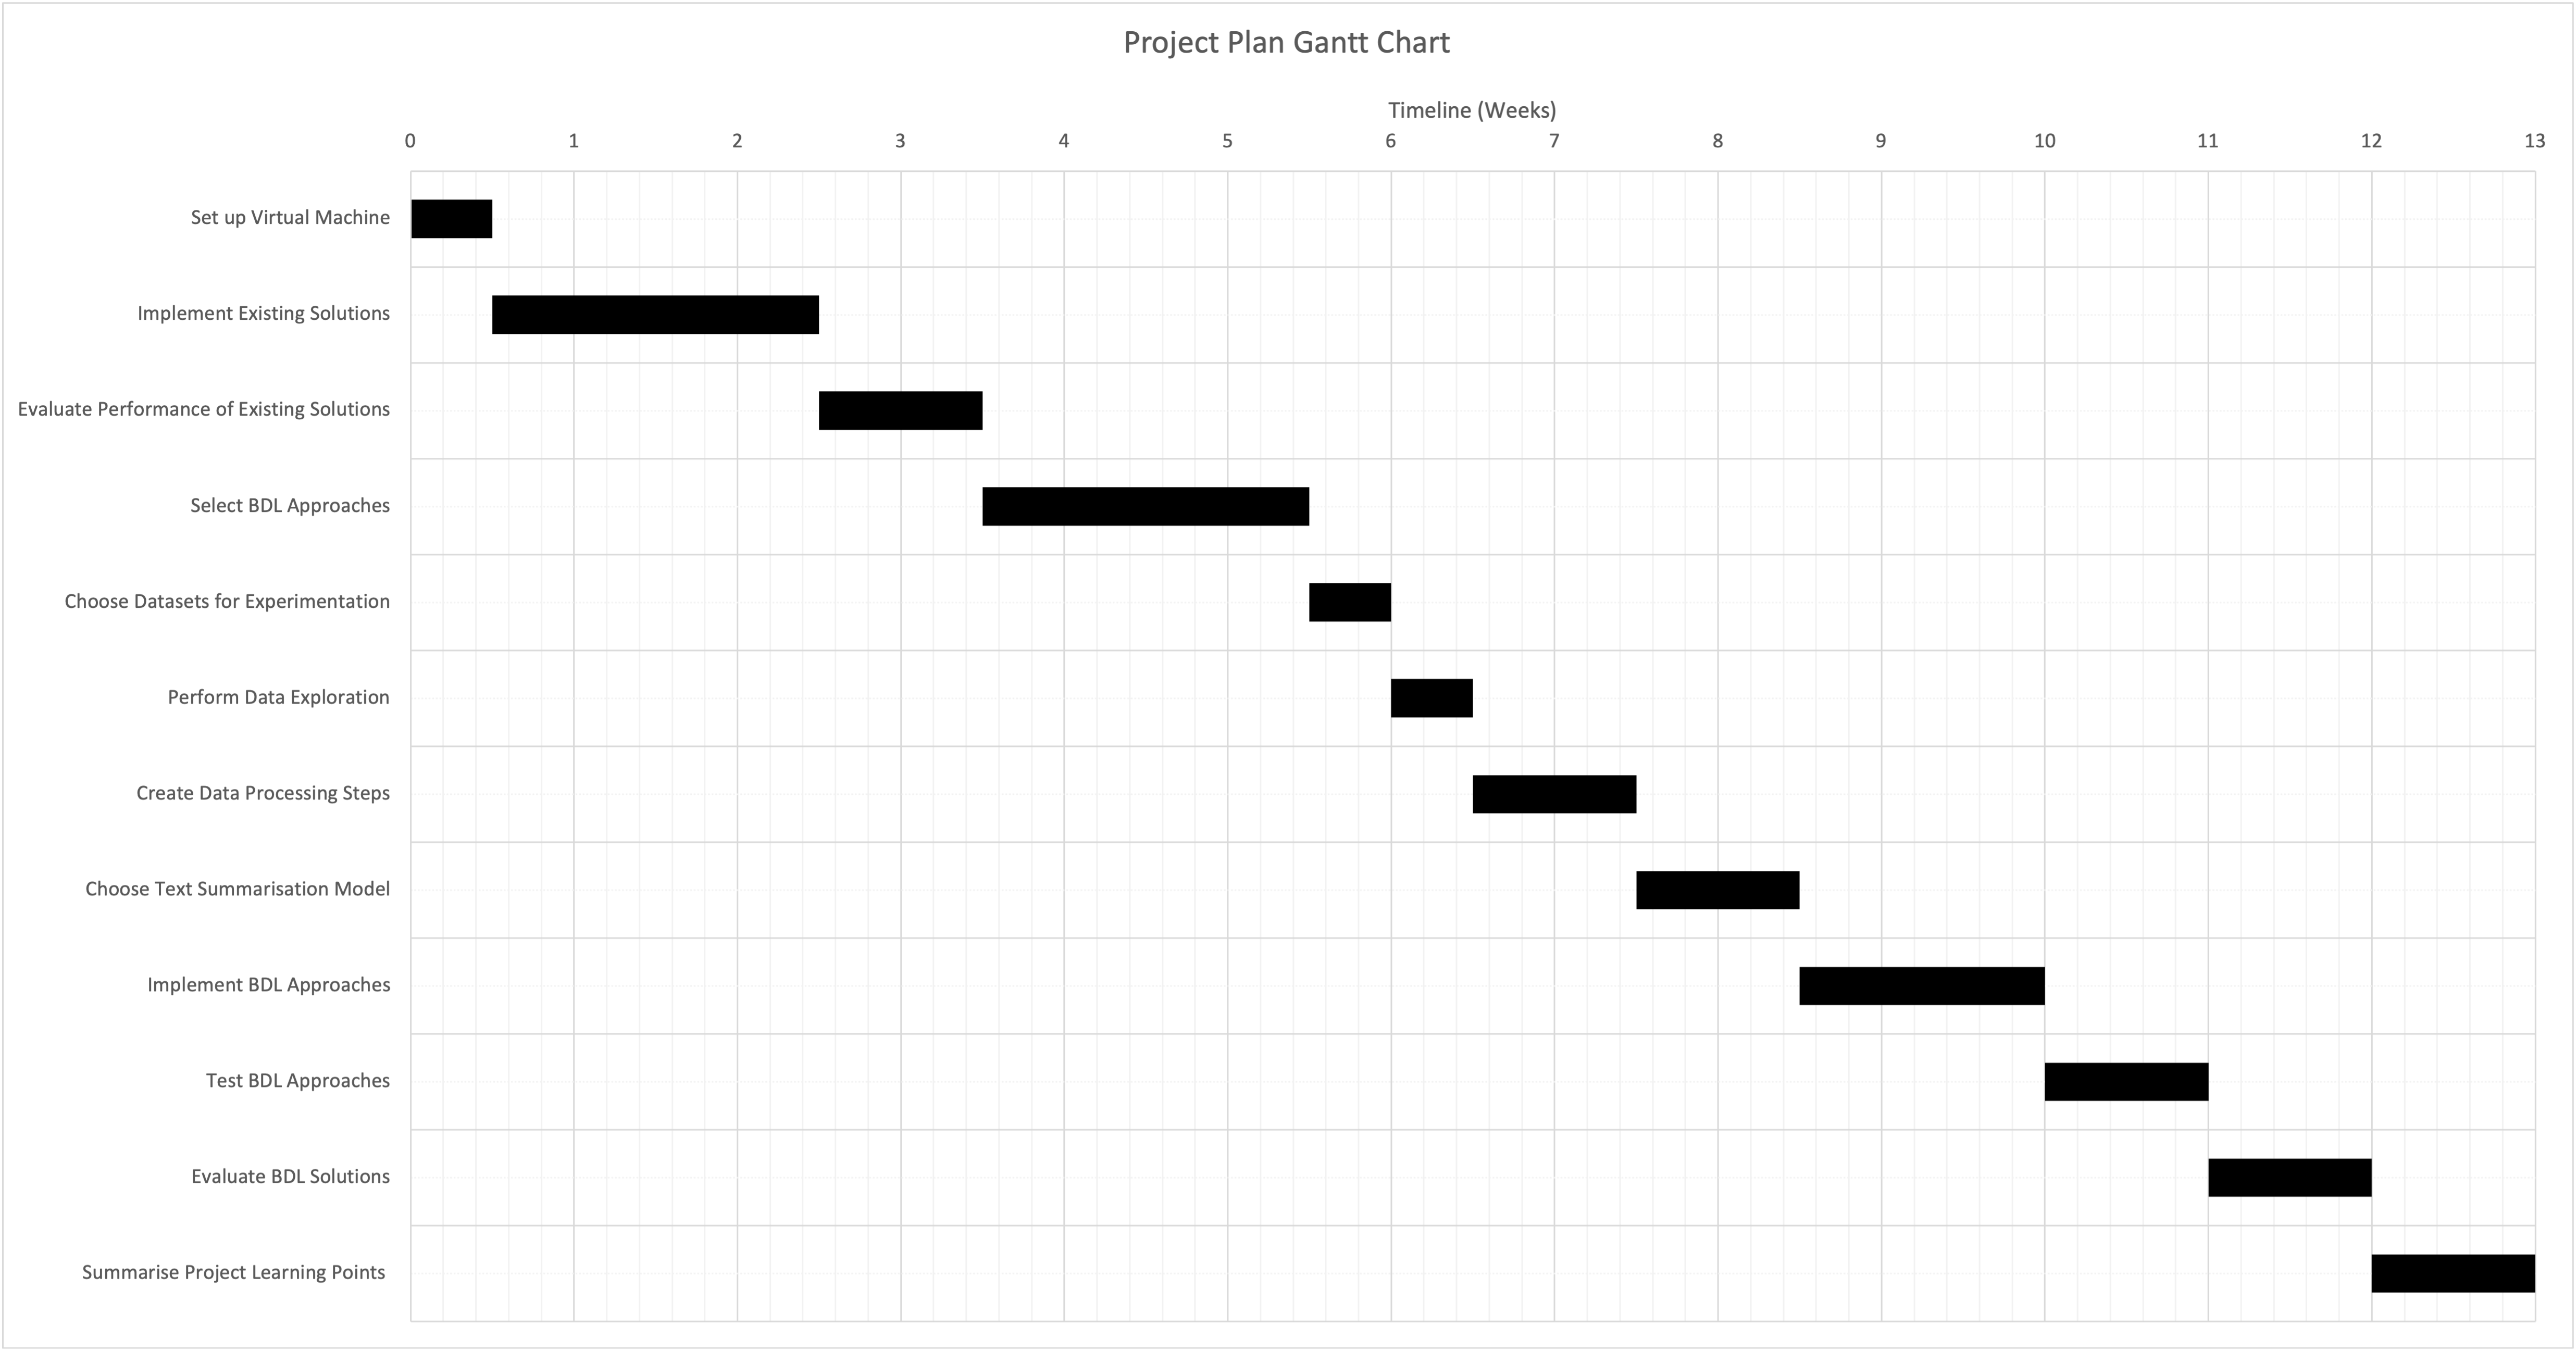
\includegraphics[width=\textwidth,height=\textheight,keepaspectratio]{Gantt.png}
		\end{center}
		
	\chapter{One-Page Risk Assessment}
		\label{appx:riskassessment}
		
		\begin{tabular}{ |p{5cm}||p{2cm}|p{2cm}|p{6cm}|  }
 			\hline
 			\multicolumn{4}{|c|}{Risk Assessment} \\
			\hline
 			Risk& Likelihood &Risk Level&Mitigations\\
 			\hline
 			Insufficient processing power for timely training on deep learning techniques   & 75\%    &50\%&  We will ensure a Virtual Machine is built to utilise the high-processing capabilities that exist virtually. We also aim to minimise the computational cost in the chosen framework. This is essential as we want the solution to be interactive. For example, using a frozen BERT model would help alleviate concerns. \\
			\hline
 			Insufficient data availability.&10\% & 90\%  & We will use publicly available data, previously used for text summarisation, passage ranking research. This is a low likelihood situation since there are many data sources available that are in common use. \\
			\hline
 			Change in research direction leads to ethical concerns since the research is active learning based. &25\% & 90\%& To evade using human annotators, we will be using noisy random selectors as our oracle. This means that an ethics review is not required; however, if there is a change in direction, we will undergo an ethics review where the time taken will be accounted for in the decision-making process.\\
			\hline
 			Due to the project being part of part-time study alongside a full-time job, there is a risk of unpredictable changes in time requirements    &20\% & 75\%& Ensure an effective usage of weekly study day as that is concretely given from work and that there is sufficient time available if tasks do overrun. We will also develop a plan outlining what needs to be achieved each week so that I constantly understand my workload.\\
 			\hline
		\end{tabular}
		
		% =============================================================================

\end{document}
